\documentclass[12pt]{scrartcl}

\usepackage[utf8]{inputenc}
\usepackage[IL2]{fontenc}
\usepackage[czech]{babel}
\usepackage{graphicx}
\usepackage{hyperref}
\usepackage{amsmath}
\usepackage{amsfonts}
\usepackage[linesnumbered]{algorithm2e}
\usepackage{enumitem}

\subject{Západočeská univerzita v\nobreakspace Plzni\\Fakulta aplikovaných věd\\KIV/KPG}
\author{Pavel Zelenka\\A16B0176P\\zelenkap@students.zcu.cz}
\date{\today}
\title{Photoshop}

\begin{document}
\maketitle
\pagenumbering{gobble}
\newpage
\pagenumbering{arabic}
\newpage
\section{Zadání}
	
\paragraph{}
Zadáním úkolu je vytvoření programu umožňujícího aplikaci efektů na\nobreakspace načteném rastrovém obrázku. 

\section{Analýza problému}
\paragraph{}
Aplikace bude mít oproti úloze na cvičení čtyři nové efekty, tj.\nobreakspace \textbf{negativ}, \textbf{sepia}, \textbf{mozaika} a \textbf{rozmazání}.

\subsection{Negativ}
\paragraph{}
\textbf{Negativ} je tonální a barevná inverze obrazu. Je-li uvažováno \texttt{8} bitů (tj. 256 tónů) na každý barevný kanál, pro získání negativu lze vzít absolutní hodnotu po odečtení konstanty \texttt{255} od každého barevného kanálu.\\\\
Získání negativní hodnoty pixelu: \\
$color = [red,\; green,\; blue]^T $ \\
$negative\_red = |red-255| $ \\
$negative\_green = |green-255| $ \\
$negative\_blue = |blue-255| $ \\
$nagative\_color = [negative\_ red,\; negative\_green,\; negative\_blue]^T $

\subsection{Sepia}
\paragraph{}
\textbf{Sepia} je jednobarevný hnědotónový obraz. V prvním kroce se obraz převede na černobílý, to se provede sečtením hodnot všech barevných kanálu a vydělením jejich počtem. Hnědého nádechu obrazu lze dosáhnout zvýšením hodnot červeného a zeleného kanálu a\nobreakspace snížením hodnoty modrého kanálu. Při\nobreakspace manipulaci s\nobreakspace tónama je nutné ošetřit, aby hodnoty byly v intervalu od \texttt{0} do \texttt{255}. V\nobreakspace případě překročení horní meze se nastaví hodnota na \texttt{255}, naopak v případě překročení dolní meze se hodnota nastaví na \texttt{0}.\\\\
Získání šedotónové hodnoty pixelu: \\
$color = [red,\; green,\; blue]^T $ \\
$gray\_tone = \frac{red + green + blue}{3} $ \\
$gray\_color = [gray\_tone,\; gray\_tone,\; gray\_tone]^T $ \\\\
Přidání sepiového efektu: \\
$\exists \; depth \in \langle -255,255 \rangle \subset{\mathbb{Z}} $ \\
$\exists \; intensity \in \langle -255,255 \rangle \subset{\mathbb{Z}} $ \\
$ gray\_color = [gray\_tone_{red},\; gray\_tone_{green},\; gray\_tone_{blue}]^T $ \\
$ sepia\_tone_{red} = gray\_tone_{red} \cdot 2 \cdot depth$ \\
$ sepia\_tone_{green} = gray\_tone_{green} \cdot depth$ \\
$ sepia\_tone_{blue} = gray\_tone_{blue} - intensity$ \\
$ sepia\_color = [sepia\_tone_{red},\; sepia\_tone_{green},\; sepia\_tone_{blue}]^T $ \\
 

\subsection{Mozaika}
\paragraph{}
\textbf{Mozaika} je obraz tvořený z kostek, počet těchto kostek může být libovolný. Přichází zde v úvahu, aby si uživatel mohl poměr rozdělení obrázku specifikovat zadáním koeficientu. Tímto koeficientem by se vynásobila šířka obrázku a výsledkem by byl počet kostek na šířku. Tato implementace vyžaduje, aby koeficent byl v intervalu od \texttt{0} do \texttt{1}. Jako minimální hodnotu koeficientu ovšem nelze zvolit \texttt{0}, obrázek by se vždy měl skládat minimálně z jedné kostky. V případě koeficientu blížící se \texttt{1} zase nastává situace, kdy počet kostek odpovídá přibližně počtu pixelů a na obrázku se neprovedou žádné změny. \\\\
Určení velikosti kostky mozaiky:\\
$\exists \; precent \in (0,1 \rangle \subset{\mathbb{R}} $\\
$\exists \; image\_width \in \mathbb{N} $\\
$ square\_side = image\_width \cdot precent $

\paragraph{}
Průchod obrázku se bude provádět vždy po násobcích velikosti čtverce, všechny pixely v tomto čtverci se přebarví na jednotnou barvu. Barvu lze zvolit více způsoby, v aplikaci se budu zabývat jednoprůchodovým způsobem, kdy je nejvhodnější zvolit barvu horního levého pixelu a dvouprůchodovým způsobem, kdy se udělá průměr barev všech pixelů ve čtverci.

\subsection{Rozmázání}
\paragraph{}
\textbf{Rozmázání} obrazu se provádí průchodem obrazu pixel po pixelu a průměrováním barvy se sousedními pixely. Problém nastává u krajních pixelů, kdy lze průměrování dělat s menším počtem sousedů nebo krajní pixely úplně vynechat.

\begin{figure}[!ht]
	\centering
	\label{obr:connectivity}
	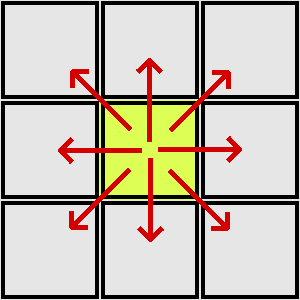
\includegraphics[width=0.25\textwidth,natwidth=1,natheight=1]{8-connectivity.pdf}
	\caption{Sousední pixely při zpracovávání obrazu (tzv. 8–connectivity)}
\end{figure}	

\paragraph{}
Při průměrování barvy lze každému pixelu dát váhu, kterou se jeho hodnota vynásobí nebo vydělí v závislosti na implementaci. V případě násobení by váha měla být v\nobreakspace intervalu od \texttt{0} do \texttt{1} (tzn. bude-li mít každý z \texttt{9} pixelů stejnou váhu, tak onou váhou bude hodnota \texttt{0.111}).

\section{Popis řešení}

\paragraph{}
Aplikace je naprogramována v jazyce \textbf{Java} s použitím grafických knihoven \textbf{JavaFX}. Algoritmy efektů jsou umístěny v samostatné třídě \emph{BasicEffects} v balíčku \emph{Effects}. Mimo nových efektů třída \emph{BasicEffects} obsahuje i efekty, které byly použity na cvičení.

\subsection{Negativ}
\paragraph{}
\begin{algorithm}[H]
	\For{každý řádek obrázku} {
		\For{každý sloupec obrázku} {
			barva = barva pixelu na pozici\;
			červená = $|$ červená složka barvy $-255\; |$\;
			zelená = $|$ zelená složka barvy $-255\; |$\;
			modrá = $|$ modrá složka barvy $-255\; |$\;
			nastav novou barvu pixelu na pozici s upravenýma složkama\;
		}
	}
 \caption{Vytvoření efektu negativu obrazu}
\end{algorithm}

\subsection{Sepia}
\paragraph{}
\begin{algorithm}[H]
\KwIn{hloubka, intenzita}
	\For{každý řádek obrázku} {
		\For{každý sloupec obrázku} {
			barva = barva pixelu na pozici\;
			červená = červená složka barvy\;
			zelená = zelená složka barvy\;
			modrá = modrá složka barvy\;
			šedá = (červená + zelená + modrá) / 3\;
			červená = šedá $+\; 2\; \cdot $ hloubka\;
			zelená = šedá $+$ hloubka\;
			modrá = šedá $-$ intenzita\;
			složky s hodnotou nad 255 nastav na 255\;
			složky s hodnotou pod 0 nastav na 0\;
			nastav novou barvu pixelu na pozici s upravenýma složkama\;
		}
	}
 \caption{Vytvoření efektu sepie obrazu}
\end{algorithm}

\subsection{Mozaika s jedním průchodem}
\paragraph{}
\begin{algorithm}[H]
\KwIn{šířka, koeficient}
	velikost čtverce  = šířka $\cdot$ koeficient\;
	\eIf{velikost čtverce $>$ 0}{
		velikost čtverce  = šířka / velikost čtverce\;
	} {
		velikost čtverce  = šířka	
	}
	\For{každý řádek obrázku, který je násobkem velikosti čtverce} {
		\For{každý sloupec obrázku, který je násobkem velikosti čtverce} {
			barva = barva pixelu na pozici\;
			\For{každý řádek čtverce} {
				\For{každý sloupec čtverce} {
					\If{procházený bod je platným bodem obrázku}{
						nastav barvu pixelu\;
					}
				}
			}
		}
	}
 \caption{Vytvoření efektu mozaika obrazu s jedním průchodem čtverce}
\end{algorithm}

\subsection{Mozaika s dvěma průchody}
\paragraph{}
\begin{algorithm}[H]
\KwIn{šířka, koeficient}
	velikost čtverce  = šířka $\cdot$ koeficient\;
	\eIf{velikost čtverce $>$ 0}{
		velikost čtverce  = šířka / velikost čtverce\;
	} {
		velikost čtverce  = šířka	
	}
	\For{každý řádek obrázku, který je násobkem velikosti čtverce} {
		\For{každý sloupec obrázku, který je násobkem velikosti čtverce} {
			počet pixelů = 0\;
			červená = 0\;
			zelená = 0\;
			modrá = 0\;
			\For{každý řádek čtverce} {
				\For{každý sloupec čtverce} {
					\If{procházený bod je platným bodem obrázku}{
						červená = červená + červená složka procházeného pixelu\;
						zelená = zelená + zelená složka procházeného pixelu\;
						modrá = modrá + modrá složka procházeného pixelu\;
						počet pixelů = počet pixelů + 1\;
					}
				}
			}
			červená = červená / počet pixelů\;
			zelená = zelená / počet pixelů\;
			modrá = modrá / počet pixelů\;
			složky s hodnotou nad 255 nastav na 255\;
			složky s hodnotou pod 0 nastav na 0\;
			vytvoř novou barvu se složkama červená, zelená, modrá\;
			\For{každý řádek čtverce} {
				\For{každý sloupec čtverce} {
					\If{procházený bod je platným bodem obrázku}{
						nastav novou barvu pixelu na procházené pozici\;
					}
				}
			}
		}
	}
 \caption{Vytvoření efektu mozaika obrazu s dvěma průchody čtverce}
\end{algorithm}

\subsection{Rozmazání}
\paragraph{}
\begin{algorithm}[H]
\KwIn{pole vah pixelů}
	\For{každý řádek obrázku mimo okrajových} {
		\For{každý sloupec obrázku mimo okrajových} {

			index váhy = 0\;
			červená = 0\;
			zelená = 0\;
			modrá = 0\;
			
			\For{řádek $-$ 1, aktuální řádek, řádek $+$ 1} {
				\For{sloupec $-$ 1, aktuální sloupec, sloupec $+$ 1} {
					\If{procházený bod je platným bodem obrázku}{
						červená = červená + červená složka pixelu / váha pixelu\;
						zelená = zelená + zelená složka pixelu / váha pixelu\;
						modrá = modrá + modrá složka pixelu / váha pixelu\;
						index váhy = index váhy + 1\;
					}
				}
			}
			složky s hodnotou nad 255 nastav na 255\;
			složky s hodnotou pod 0 nastav na 0\;	
			nastav novou barvu pixelu na pozici s upravenýma složkama\;
		}
	}
 \caption{Vytvoření efektu negativu obrazu}
\end{algorithm}

\newpage
\section{Uživatelská dokumentace}
\paragraph{}
Aplikace byla testována na operačním systému \textbf{GNU/Linux} s nainstalovaným \textbf{Java Development Kit} ve\nobreakspace verzi\nobreakspace 1.8.0\_162. Spouštěcí soubor aplikace \texttt{SimplePhotoshop.jar} se nachází ve složce \emph{App}.

\paragraph{}
Po\nobreakspace spuštění aplikace se\nobreakspace zobrazí okno s\nobreakspace výchozím obrázkem. V pravém panelu se nachází tlačítka efektů \textbf{Blur} pro rozmazání, \textbf{Black \& White} pro černobílý obraz, \textbf{Emboss} pro\nobreakspace tepaný obraz, \textbf{Mosaic} pro mozaiku, \textbf{Negative} pro negativ a \textbf{Sepia} pro\nobreakspace efekt sepie. Pro\nobreakspace aplikaci efektu je vždy nutné kliknout na potvrzovací tlačítko \textbf{Apply}. Obraz lze vždy vrátit o jeden krok zpět tlačítkem \textbf{Undo}. Obnovit původní obrázek lze tlačítkem \textbf{Reset}.

\paragraph{}
Skrze tlačítko \textbf{Open} v nabídce \textbf{File} lze načíst obrázky ve formátu \texttt{PNG}, \texttt{JPG} a \texttt{BMP}. Ve\nobreakspace stejné nabídce skrze tlačítko \textbf{Save As...} lze obrázek uložit ve formátu \texttt{PNG}.

\paragraph{}
Ve spodním panelu je zobrazeno rozlišení načteného obrázku.

\begin{figure}[!ht]
	\centering
	\label{obr:aplikace}
	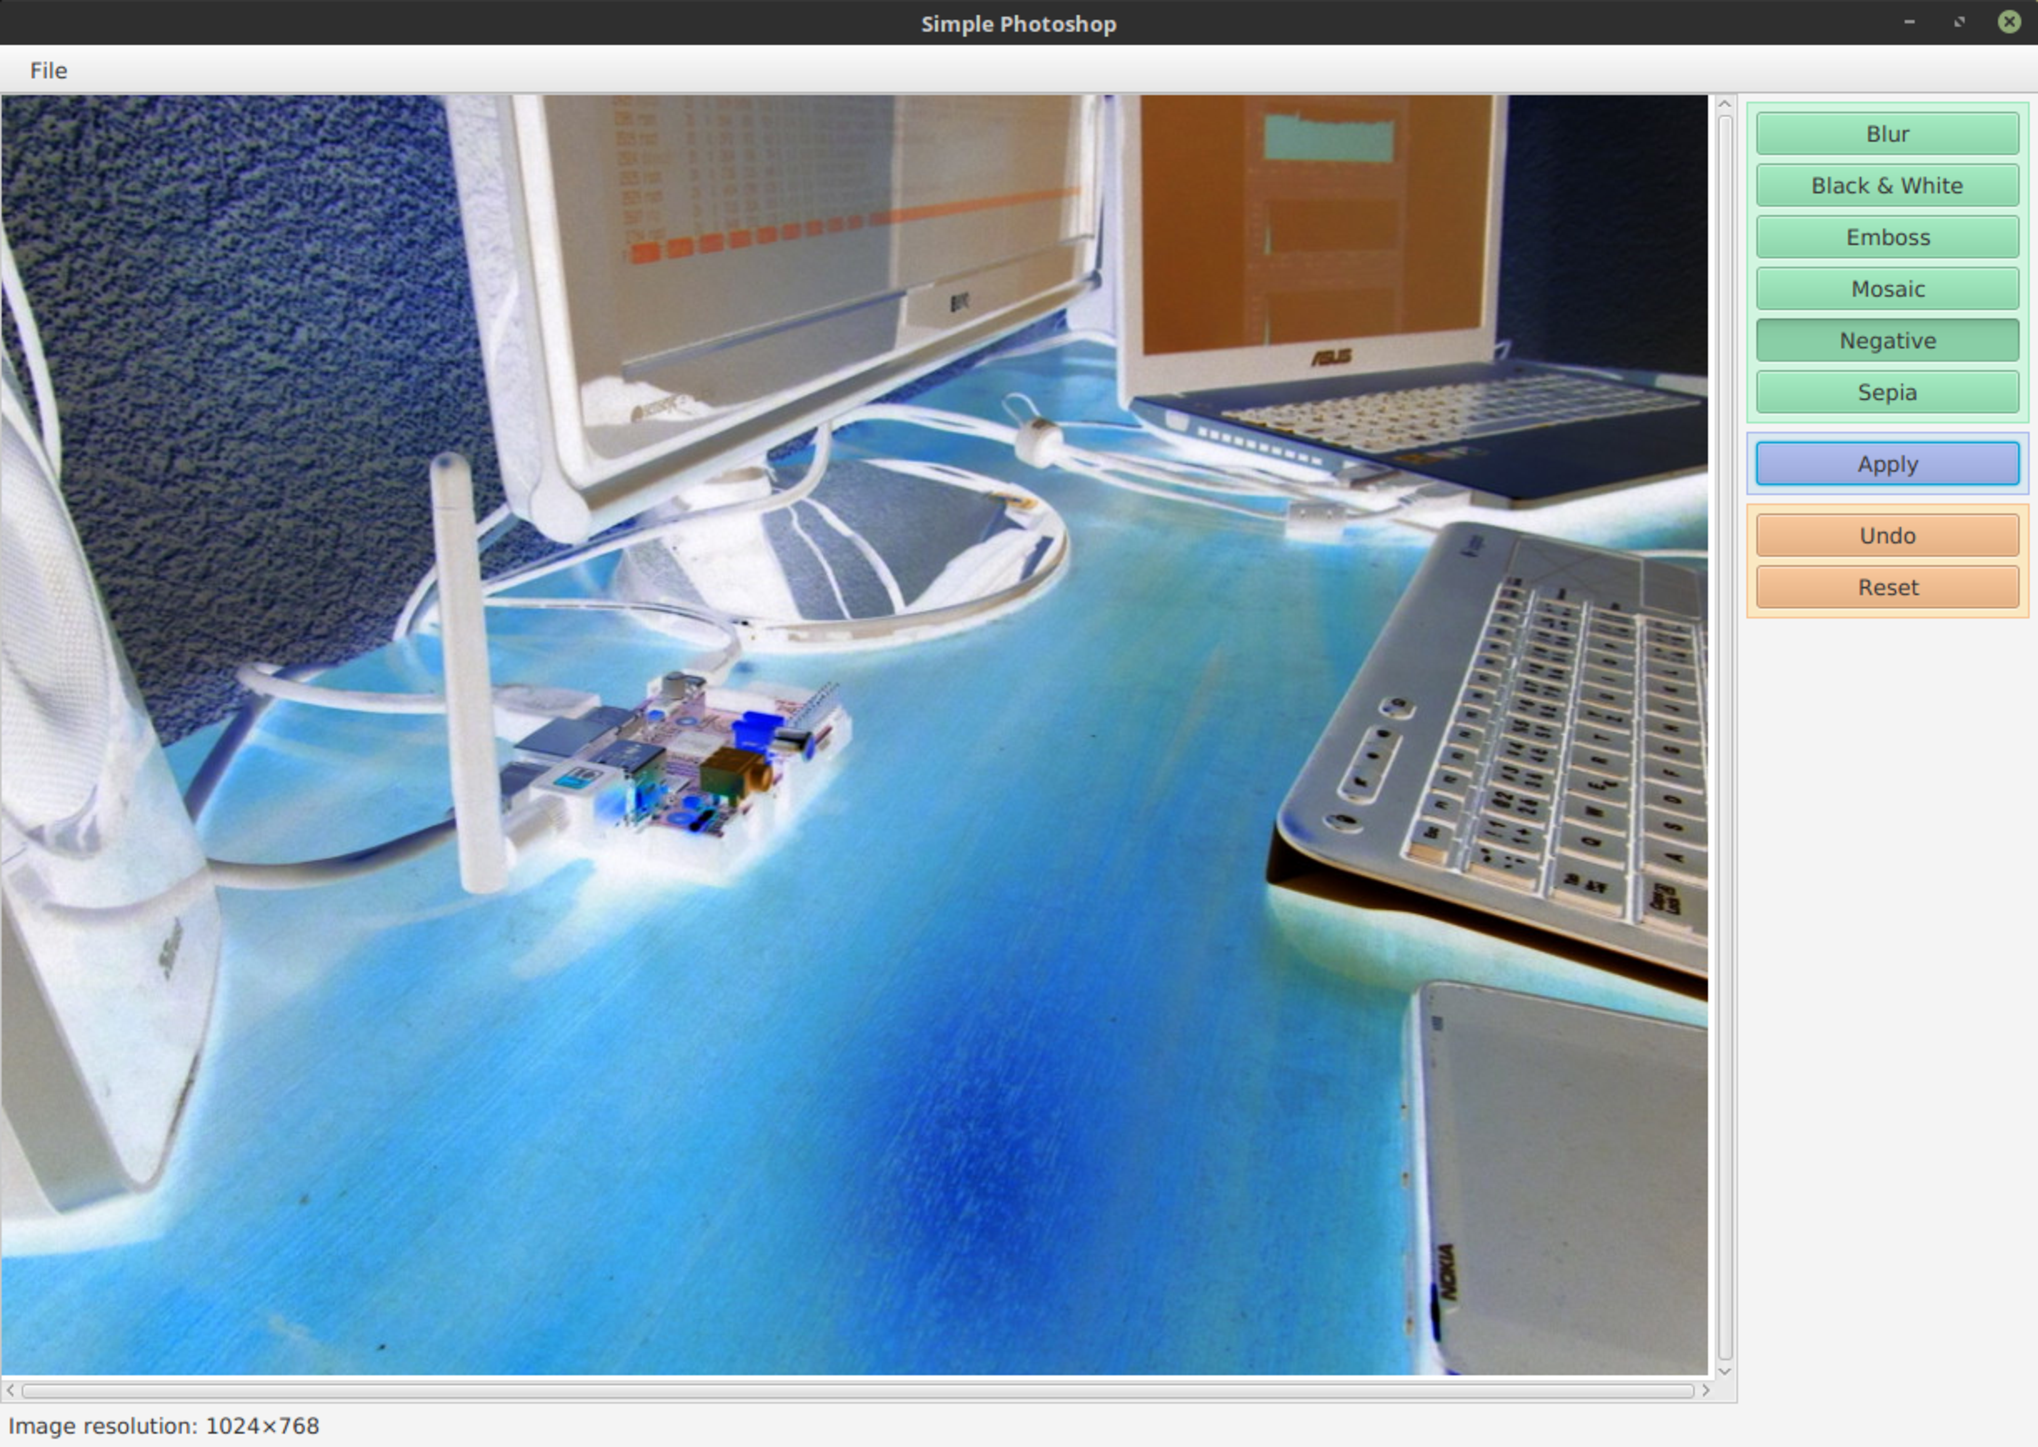
\includegraphics[width=0.9\textwidth,natwidth=1,natheight=1]{app_gui.pdf}
	\caption{Okno aplikace}
\end{figure}	

\newpage
\section{Závěr}
\paragraph{}
Aplikaci jsem testoval na obrázku \textsf{lena.bmp}, tedy na shodném obrázku jako byl použit na cvičení. Aplikaci efektů na obrázku o rozměrech \texttt{512 $\times$ 512} pixelů jsem testoval na notebooku s procesorem \texttt{Intel Core i7-3610QM} a na operačním systému \texttt{GNU/Linux}.

\subsection{Výsledky pro negativ}

\begin{figure}[!ht]
	\centering
	\label{obr:negativ}
	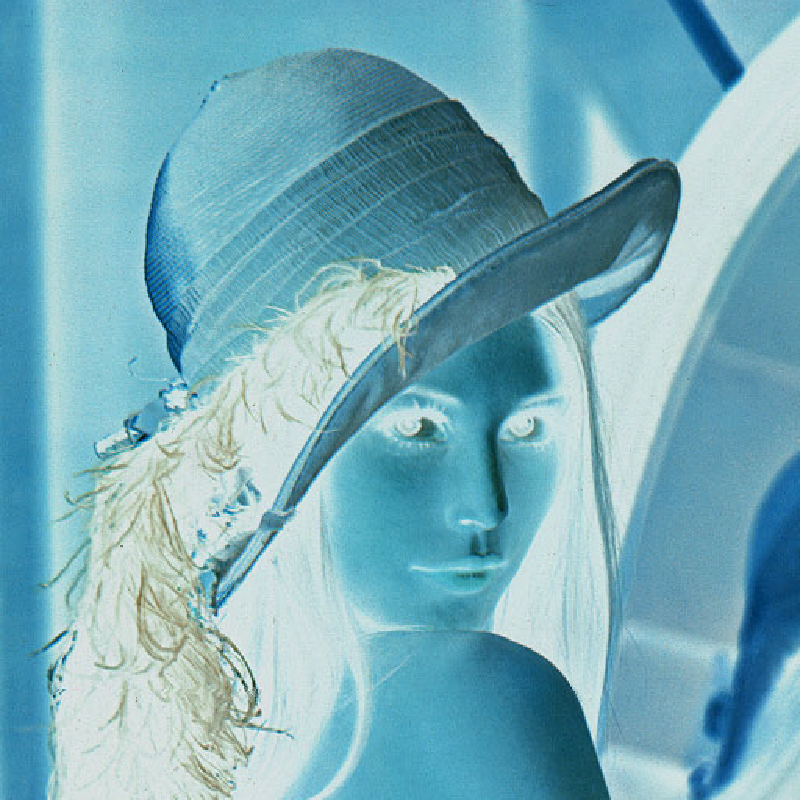
\includegraphics[width=0.7\textwidth,natwidth=1,natheight=1]{negative.pdf}
	\caption{Efekt negativ na výchozím obrázku}
\end{figure}	

\begin{center}
  \begin{tabular}{ | l | r | }
    \hline
    počet pokusů: & 5 \\ \hline
    nejlepší čas: & 31 ms \\ \hline
    nejhorší čas: & 48 ms \\ \hline
    průměrný čas: & 36 ms \\
    \hline
  \end{tabular}
\end{center}

\newpage
\subsection{Výsledky pro sepii}

\begin{figure}[!ht]
	\centering
	\label{obr:sepia}
	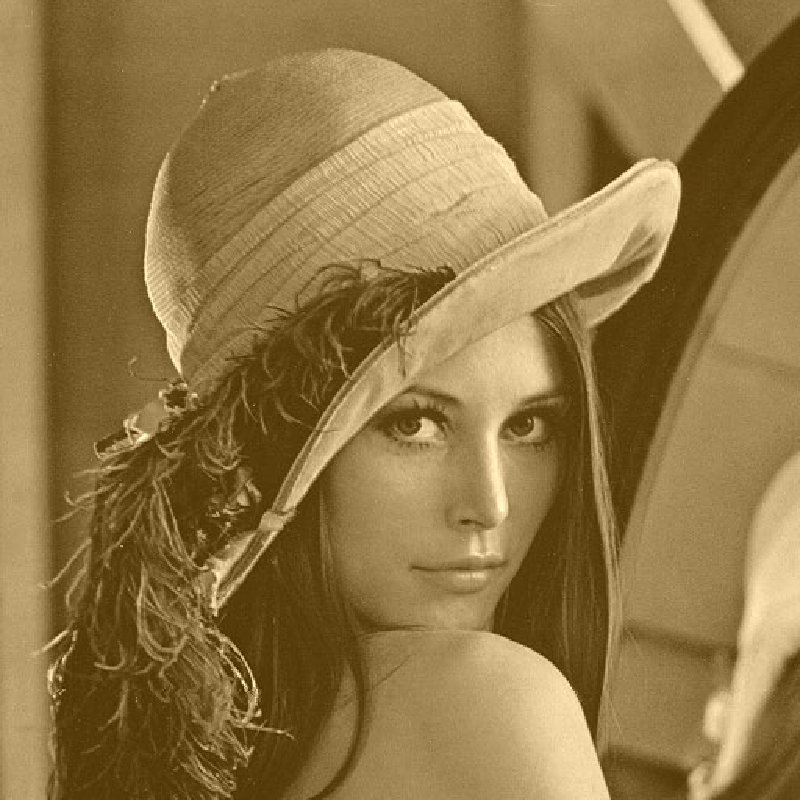
\includegraphics[width=0.7\textwidth,natwidth=1,natheight=1]{sepia.pdf}
	\caption{Efekt sepia na výchozím obrázku}
\end{figure}	

\begin{center}
  \begin{tabular}{ | l | r | }
    \hline
    počet pokusů: & 5 \\ \hline
    nejlepší čas: & 27 ms \\ \hline
    nejhorší čas: & 34 ms \\ \hline
    průměrný čas: & 31 ms \\
    \hline
  \end{tabular}
\end{center}

\newpage
\subsection{Výsledky pro mozaiku s jedním průchodem}

\begin{figure}[!ht]
	\centering
	\label{obr:mosaic}
	
\includegraphics[width=0.7\textwidth,natwidth=1,natheight=1]{mosaic_simple.pdf}
	\caption{Efekt mazaika s jedním průchodem na výchozím obrázku}
\end{figure}	

\begin{center}
  \begin{tabular}{ | l | r | }
    \hline
    počet pokusů: & 5 \\ \hline
    nejlepší čas: & 7 ms \\ \hline
    nejhorší čas: & 16 ms \\ \hline
    průměrný čas: & 13 ms \\
    \hline
  \end{tabular}
\end{center}

\newpage
\subsection{Výsledky pro mozaiku s dvěma průchody}

\begin{figure}[!ht]
	\centering
	\label{obr:mosaicdouble}
	
\includegraphics[width=0.7\textwidth,natwidth=1,natheight=1]{mosaic_double.pdf}
	\caption{Efekt mazaika s dvěma průchody na výchozím obrázku}
\end{figure}	

\begin{center}
  \begin{tabular}{ | l | r | }
    \hline
    počet pokusů: & 5 \\ \hline
    nejlepší čas: & 16 ms \\ \hline
    nejhorší čas: & 29 ms \\ \hline
    průměrný čas: & 22 ms \\
    \hline
  \end{tabular}
\end{center}

\newpage
\subsection{Výsledky pro rozmazání}

\begin{figure}[!ht]
	\centering
	\label{obr:blur}
	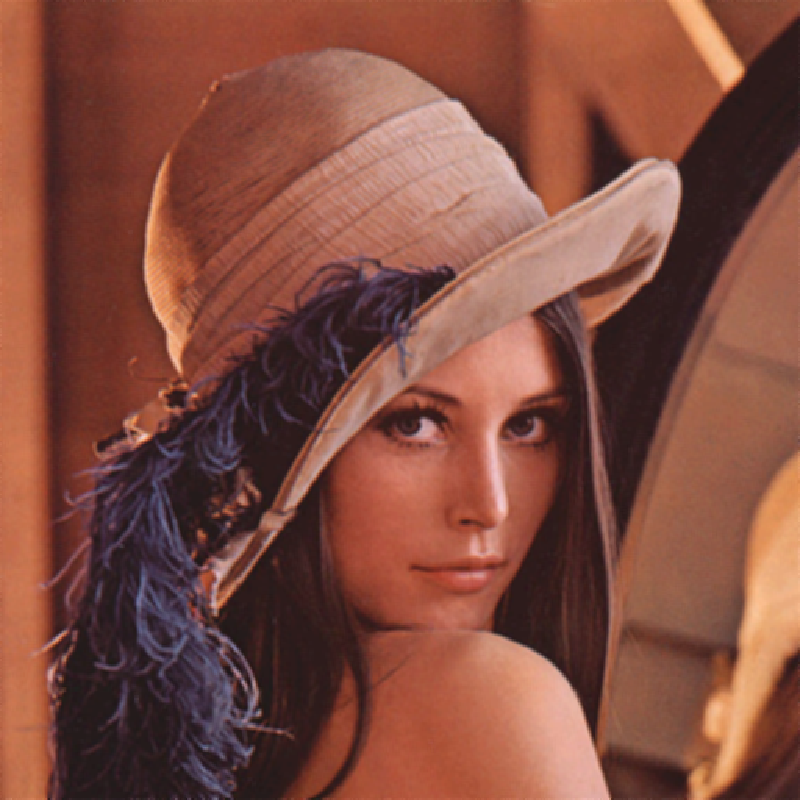
\includegraphics[width=0.7\textwidth,natwidth=1,natheight=1]{blur.pdf}
	\caption{Efekt rozmazání na výchozím obrázku}
\end{figure}	

\begin{center}
  \begin{tabular}{ | l | r | }
    \hline
    počet pokusů: & 5 \\ \hline
    nejlepší čas: & 126 ms \\ \hline
    nejhorší čas: & 134 ms \\ \hline
    průměrný čas: & 128 ms \\
    \hline
  \end{tabular}
\end{center}

\section{Reference}

Blurring for Beginners – JH Labs. [online]. Dostupné z: \href{http://www.jhlabs.com/ip/blurring.html}{www.jhlabs.com/ip/blurring.html}

\end{document}
